% Copie LaTeX de README.md (projet Assurance de risque), générée par
% generation/generer_latex.py. Compilation : pdflatex, xelatex ou lualatex
% (deux passes pour la table des matières), depuis ce dossier.
% Options for packages loaded elsewhere

\PassOptionsToPackage{unicode}{hyperref}

\PassOptionsToPackage{hyphens}{url}

\PassOptionsToPackage{dvipsnames,svgnames,x11names}{xcolor}

\documentclass[

  french,

  10pt,

  a4paper,

]{article}

\usepackage{xcolor}

\usepackage[margin=2cm]{geometry}

\usepackage{amsmath,amssymb}

\setcounter{secnumdepth}{-\maxdimen} % remove section numbering

\usepackage{iftex}

\ifPDFTeX

  \usepackage[T1]{fontenc}

  \usepackage[utf8]{inputenc}

  \usepackage{textcomp} % provide euro and other symbols

\else % if luatex or xetex

  \usepackage{unicode-math} % this also loads fontspec

  \defaultfontfeatures{Scale=MatchLowercase}

  \defaultfontfeatures[\rmfamily]{Ligatures=TeX,Scale=1}

\fi

\usepackage{lmodern}

\ifPDFTeX\else

  % xetex/luatex font selection

\fi

% Use upquote if available, for straight quotes in verbatim environments

\IfFileExists{upquote.sty}{\usepackage{upquote}}{}

\IfFileExists{microtype.sty}{% use microtype if available

  \usepackage[]{microtype}

  \UseMicrotypeSet[protrusion]{basicmath} % disable protrusion for tt fonts

}{}

\makeatletter

\@ifundefined{KOMAClassName}{% if non-KOMA class

  \IfFileExists{parskip.sty}{%

    \usepackage{parskip}

  }{% else

    \setlength{\parindent}{0pt}

    \setlength{\parskip}{6pt plus 2pt minus 1pt}}

}{% if KOMA class

  \KOMAoptions{parskip=half}}

\makeatother

\usepackage{longtable,booktabs,array}

\newcounter{none} % for unnumbered tables

\usepackage{calc} % for calculating minipage widths

% Correct order of tables after \paragraph or \subparagraph

\usepackage{etoolbox}

\makeatletter

\patchcmd\longtable{\par}{\if@noskipsec\mbox{}\fi\par}{}{}

\makeatother

% Allow footnotes in longtable head/foot

\IfFileExists{footnotehyper.sty}{\usepackage{footnotehyper}}{\usepackage{footnote}}

\makesavenoteenv{longtable}

\usepackage{graphicx}

\makeatletter

\newsavebox\pandoc@box

\newcommand*\pandocbounded[1]{% scales image to fit in text height/width

  \sbox\pandoc@box{#1}%

  \Gscale@div\@tempa{\textheight}{\dimexpr\ht\pandoc@box+\dp\pandoc@box\relax}%

  \Gscale@div\@tempb{\linewidth}{\wd\pandoc@box}%

  \ifdim\@tempb\p@<\@tempa\p@\let\@tempa\@tempb\fi% select the smaller of both

  \ifdim\@tempa\p@<\p@\scalebox{\@tempa}{\usebox\pandoc@box}%

  \else\usebox{\pandoc@box}%

  \fi%

}

% Set default figure placement to htbp

\def\fps@figure{htbp}

\makeatother

\ifLuaTeX

\usepackage[bidi=basic,shorthands=off]{babel}

\else

\usepackage[bidi=default,shorthands=off]{babel}

\fi

\ifLuaTeX

  \usepackage{selnolig} % disable illegal ligatures

\fi

\setlength{\emergencystretch}{3em} % prevent overfull lines

\providecommand{\tightlist}{%

  \setlength{\itemsep}{0pt}\setlength{\parskip}{0pt}}

% En-tête ajouté au modèle LaTeX de Pandoc pour les copies des README du projet.

% N'utilise que des extensions standard (float, etoolbox), présentes dans TeX Live,

% MiKTeX et Overleaf.

\usepackage{float}

\floatplacement{figure}{H}               % chaque figure reste à sa place dans le texte

\usepackage{etoolbox}

\AtBeginEnvironment{longtable}{\small}   % tableaux en petit corps

\setlength{\tabcolsep}{4pt}

\makeatletter

\renewcommand{\verbatim@font}{\small\ttfamily}  % blocs de code (commandes, arborescence)

\makeatother

\usepackage{bookmark}

\IfFileExists{xurl.sty}{\usepackage{xurl}}{} % add URL line breaks if available

\urlstyle{same}

\hypersetup{

  pdftitle={Étape 1.1 --- Analyse de la qualité des données},

  pdflang={fr},

  colorlinks=true,

  linkcolor={blue},

  filecolor={Maroon},

  citecolor={Blue},

  urlcolor={blue},

  pdfcreator={LaTeX via pandoc}}



\title{Étape 1.1 --- Analyse de la qualité des données}

\author{}

\date{}



\begin{document}

\maketitle



{

\hypersetup{linkcolor=black}

\setcounter{tocdepth}{3}

\tableofcontents

}

\begin{quote}

\textbf{Énoncé (1.1)} : évaluer la qualité des données et identifier les variables non pertinentes (identifiants, variables redondantes ou de variabilité insuffisante) ; analyser les valeurs manquantes et proposer une stratégie (suppression, imputation, modalité spécifique) ; vérifier la cohérence (doublons, valeurs incohérentes, plages de valeurs, variables constantes) et justifier les décisions.

\end{quote}



\section{Exécution}



\begin{verbatim}

.venv\Scripts\python.exe partie1_donnees\1.1_qualite\etape_1_1_qualite.py

\end{verbatim}



\textbf{Notebook} (déjà exécuté : tableaux et figures visibles sans rien relancer) : \href{etape_1_1_qualite.ipynb}{\texttt{etape\_1\_1\_qualite.ipynb}}. \textbf{Version LaTeX} de ce document : \texttt{README.tex}.



{\def\LTcaptype{none} % do not increment counter

\begin{longtable}[]{@{}

  >{\raggedright\arraybackslash}p{(\linewidth - 2\tabcolsep) * \real{0.5000}}

  >{\raggedright\arraybackslash}p{(\linewidth - 2\tabcolsep) * \real{0.5000}}@{}}

\toprule\noalign{}

\begin{minipage}[b]{\linewidth}\raggedright

Entrée

\end{minipage} & \begin{minipage}[b]{\linewidth}\raggedright

Sortie principale

\end{minipage} \\

\midrule\noalign{}

\endhead

\bottomrule\noalign{}

\endlastfoot

\texttt{sources/InsuranceData.xlsx} & \textbf{\texttt{resultats/donnees\_qualite.csv}} (et \texttt{.xlsx}) : 4 074 individus \ensuremath{\times} 59 colonnes, nettoyé et typé \\

\end{longtable}

}



Les règles de conversion du texte libre sont dans \texttt{commun/outils.py} (fonctions \texttt{texte\_vers\_*}).



\begin{center}\rule{0.5\linewidth}{0.5pt}\end{center}



\section{1. Identifiants et variables techniques}



{\def\LTcaptype{none} % do not increment counter

\begin{longtable}[]{@{}

  >{\raggedright\arraybackslash}p{(\linewidth - 4\tabcolsep) * \real{0.3333}}

  >{\raggedright\arraybackslash}p{(\linewidth - 4\tabcolsep) * \real{0.3333}}

  >{\raggedright\arraybackslash}p{(\linewidth - 4\tabcolsep) * \real{0.3333}}@{}}

\toprule\noalign{}

\begin{minipage}[b]{\linewidth}\raggedright

Variable

\end{minipage} & \begin{minipage}[b]{\linewidth}\raggedright

Constat

\end{minipage} & \begin{minipage}[b]{\linewidth}\raggedright

Décision

\end{minipage} \\

\midrule\noalign{}

\endhead

\bottomrule\noalign{}

\endlastfoot

\texttt{id} (colonne « N ») & 4 076 valeurs distinctes, de 1 à 4 076, sans trou : c'est le numéro d'ordre de saisie & \textbf{Conservé comme clé} pour suivre chaque individu d'une étape à l'autre, \textbf{exclu de tous les modèles} : il ne porte aucune information sur le risque, et un modèle pourrait s'en servir à tort pour capter l'ordre de saisie (enquêteur, quartier\ldots). \\

\end{longtable}

}



Le fichier ne contient pas d'autre variable technique (date de saisie, code enquêteur\ldots).



\section{2. Mise au format (préalable aux contrôles)}



\subsection{2.1 Réponses multiples}



Dans 24 variables, une même cellule contient parfois plusieurs modalités (par exemple « Masculin Féminin »). \textbf{Règle : on garde la première modalité citée}, supposée être la réponse principale. Au total, \textbf{1 305 cellules} ont été résolues ainsi.



{\def\LTcaptype{none} % do not increment counter

\begin{longtable}[]{@{}lrr@{}}

\toprule\noalign{}

Variable & Cellules multiples & \% \\

\midrule\noalign{}

\endhead

\bottomrule\noalign{}

\endlastfoot

secteur & 355 & 8,7 \\

type\_recours & 222 & 5,4 \\

source\_electricite & 193 & 4,7 \\

energie\_cuisine & 190 & 4,7 \\

revenu & 97 & 2,4 \\

transport\_travail & 88 & 2,2 \\

activite\_conjoint & 37 & 0,9 \\

17 autres variables & 1 à 32 & \textless{} 0,8 \\

\end{longtable}

}



\subsection{2.2 Recodage des modalités}



Les 35 variables qualitatives ont été recodées en libellés courts en français. Les numéros de modalité et les traductions malgaches sont supprimés : \emph{Eny} \ensuremath{\rightarrow} Oui, \emph{Tsia} \ensuremath{\rightarrow} Non, \emph{Tompon-trano} \ensuremath{\rightarrow} Propriétaire, \emph{Manofa trano} \ensuremath{\rightarrow} Locataire, \emph{Hazo kitay} \ensuremath{\rightarrow} Bois, \emph{Tongotra} \ensuremath{\rightarrow} À pied\ldots{} Les tranches de revenu deviennent \texttt{\textless{}100k}, \texttt{100-200k}, \ldots, \texttt{\textgreater{}1M} (Ariary par mois). La table de correspondance complète figure dans \texttt{tables/recodage\_modalites.csv}.



\subsection{2.3 Conversion du texte libre en nombres}



{\def\LTcaptype{none} % do not increment counter

\begin{longtable}[]{@{}

  >{\raggedright\arraybackslash}p{(\linewidth - 14\tabcolsep) * \real{0.1250}}

  >{\raggedleft\arraybackslash}p{(\linewidth - 14\tabcolsep) * \real{0.1250}}

  >{\raggedleft\arraybackslash}p{(\linewidth - 14\tabcolsep) * \real{0.1250}}

  >{\raggedleft\arraybackslash}p{(\linewidth - 14\tabcolsep) * \real{0.1250}}

  >{\raggedleft\arraybackslash}p{(\linewidth - 14\tabcolsep) * \real{0.1250}}

  >{\raggedleft\arraybackslash}p{(\linewidth - 14\tabcolsep) * \real{0.1250}}

  >{\raggedleft\arraybackslash}p{(\linewidth - 14\tabcolsep) * \real{0.1250}}

  >{\raggedleft\arraybackslash}p{(\linewidth - 14\tabcolsep) * \real{0.1250}}@{}}

\toprule\noalign{}

\begin{minipage}[b]{\linewidth}\raggedright

Variable

\end{minipage} & \begin{minipage}[b]{\linewidth}\raggedleft

Nombre pur

\end{minipage} & \begin{minipage}[b]{\linewidth}\raggedleft

Zéro codé (\texttt{O}, \texttt{00}, \texttt{P})

\end{minipage} & \begin{minipage}[b]{\linewidth}\raggedleft

Phrase = « rien »

\end{minipage} & \begin{minipage}[b]{\linewidth}\raggedleft

Nombre extrait d'une phrase

\end{minipage} & \begin{minipage}[b]{\linewidth}\raggedleft

Fourchette

\end{minipage} & \begin{minipage}[b]{\linewidth}\raggedleft

Calcul

\end{minipage} & \begin{minipage}[b]{\linewidth}\raggedleft

Inexploitable \ensuremath{\rightarrow} manquant

\end{minipage} \\

\midrule\noalign{}

\endhead

\bottomrule\noalign{}

\endlastfoot

anciennete\_emploi & 2 986 & 1 & 0 & 968 & 7 & 14 & 85 \\

distance\_travail & 1 667 & 672 & 77 & 1 199 & 181 & 0 & 250 \\

heures\_jour & 3 305 & 0 & 4 & 586 & 64 & 0 & 106 \\

jours\_semaine & 3 287 & 2 & 4 & 709 & 12 & 0 & 50 \\

jours\_arret & 2 368 & 528 & 172 & 814 & 8 & 5 & 12 \\

distance\_soins & 1 460 & 1 479 & 16 & 896 & 19 & 0 & 14 \\

cout\_consultation & 945 & 2 826 & 6 & 30 & 1 & 2 & 8 \\

cout\_hospitalisation & 195 & 3 569 & 7 & 6 & 0 & 0 & 1 \\

cout\_medicaments & 2 845 & 861 & 46 & 69 & 4 & 3 (+ 2 corrigés à la main) & 11 \\

cout\_deplacement & 511 & 3 271 & 7 & 13 & 0 & 2 & 2 \\

cout\_alimentation & 412 & 3 236 & 35 & 16 & 2 & 2 (+ 1) & 78 \\

cout\_autres & 171 & 3 558 & 5 & 17 & 0 & 5 (+ 1) & 3 \\

\end{longtable}

}



\textbf{Principales règles appliquées} (détail dans les fonctions \texttt{texte\_vers\_*} de \texttt{commun/outils.py}) :



\begin{itemize}

\tightlist

\item

  \textbf{Montants} : \texttt{20\ 000} \ensuremath{\rightarrow} 20000 ; \texttt{30000ar} \ensuremath{\rightarrow} 30000 ; \texttt{8000\ensuremath{\times}2:16000} \ensuremath{\rightarrow} 16000 (résultat du calcul) ; \texttt{11000\ \textasciitilde{}\ 15000} \ensuremath{\rightarrow} 13000 (milieu de la fourchette) ; \texttt{15000\ (\ldots{})\ +\ 3000} \ensuremath{\rightarrow} 18000 ; \texttt{2\ million} \ensuremath{\rightarrow} 2 000 000. Sinon, on retient le plus grand nombre cité, car les petits nombres sont des quantités ou des durées (\texttt{10000\ (2000\ isanandro)} \ensuremath{\rightarrow} 10000).

\item

  \textbf{Saisies signifiant « aucune dépense » \ensuremath{\rightarrow} 0} : \texttt{Tsy\ nisy} (rien), \texttt{Tambavy} / \texttt{Evoka} / \texttt{Ravina} (tisane, inhalation, feuilles : remèdes traditionnels gratuits), \texttt{Nadeha\ tongotra} (à pied), \texttt{Tsa\ niova\ ny\ sakafo} (alimentation inchangée), \texttt{Nahazo\ prise\ en\ charge} (pris en charge par un tiers).

\item

  \textbf{Inexploitable \ensuremath{\rightarrow} manquant} : \texttt{Tsy\ tadidy} (je ne me souviens pas), \texttt{Tena\ volabe\ no\ lany} (« beaucoup d'argent »), \texttt{Miovaova} / \texttt{Arakaraka} (« variable », « ça dépend »).

\item

  \textbf{Distances} : \texttt{1km} \ensuremath{\rightarrow} 1 ; \texttt{500\ m} \ensuremath{\rightarrow} 0,5 ; \texttt{0-3km} \ensuremath{\rightarrow} 1,5 ; un nombre sans unité \ensuremath{\geq} 50 est lu en mètres ; travail à domicile \ensuremath{\rightarrow} 0 ; une durée en minutes (\texttt{5mn}) \ensuremath{\rightarrow} manquant.

\item

  \textbf{Durées d'arrêt (jours)} : \texttt{Herinandro} (une semaine) \ensuremath{\rightarrow} 7 ; \texttt{Tapabolana} (quinze jours) \ensuremath{\rightarrow} 15 ; \texttt{Ray\ volana} (un mois) \ensuremath{\rightarrow} 30 ; \texttt{1\ mois\ +\ 15\ jours} \ensuremath{\rightarrow} 45 ; \texttt{Niasa\ ihany} (a continué à travailler) \ensuremath{\rightarrow} 0.

\item

  \textbf{Ancienneté (années)} : \texttt{4taona} \ensuremath{\rightarrow} 4 ; \texttt{6\ mois} \ensuremath{\rightarrow} 0,5 ; \texttt{Depuis\ 2007} \ensuremath{\rightarrow} 19 (année d'enquête 2026) ; \texttt{Depuis\ l\textquotesingle{}enfance} \ensuremath{\rightarrow} manquant.

\end{itemize}



Limite : un montant donné « par jour » sans durée (\texttt{5000\ par\ jours}) est gardé tel quel, ce qui sous-estime le coût. Une dizaine de cas sont concernés.



\subsection{2.4 Construction du coût total (variable de sévérité)}



\texttt{cout\_total} = somme des six postes G.1 à G.6. Un poste vide à côté de postes renseignés compte pour 0 (aucune dépense déclarée) ; si les six postes sont vides, le coût total est manquant.



{\def\LTcaptype{none} % do not increment counter

\begin{longtable}[]{@{}

  >{\raggedright\arraybackslash}p{(\linewidth - 10\tabcolsep) * \real{0.1667}}

  >{\raggedleft\arraybackslash}p{(\linewidth - 10\tabcolsep) * \real{0.1667}}

  >{\raggedleft\arraybackslash}p{(\linewidth - 10\tabcolsep) * \real{0.1667}}

  >{\raggedleft\arraybackslash}p{(\linewidth - 10\tabcolsep) * \real{0.1667}}

  >{\raggedleft\arraybackslash}p{(\linewidth - 10\tabcolsep) * \real{0.1667}}

  >{\raggedleft\arraybackslash}p{(\linewidth - 10\tabcolsep) * \real{0.1667}}@{}}

\toprule\noalign{}

\begin{minipage}[b]{\linewidth}\raggedright

Poste

\end{minipage} & \begin{minipage}[b]{\linewidth}\raggedleft

Renseigné

\end{minipage} & \begin{minipage}[b]{\linewidth}\raggedleft

Dépense \textgreater{} 0

\end{minipage} & \begin{minipage}[b]{\linewidth}\raggedleft

Médiane si \textgreater{} 0 (Ar)

\end{minipage} & \begin{minipage}[b]{\linewidth}\raggedleft

Moyenne si \textgreater{} 0 (Ar)

\end{minipage} & \begin{minipage}[b]{\linewidth}\raggedleft

Maximum (Ar)

\end{minipage} \\

\midrule\noalign{}

\endhead

\bottomrule\noalign{}

\endlastfoot

Consultation & 3 810 & 26 \% & 10 000 & 14 610 & 500 000 \\

Hospitalisation & 3 777 & 5 \% & 10 000 & 67 289 & 7 000 000 \\

Médicaments & 3 830 & \textbf{76 \%} & 10 000 & 26 450 & 1 600 000 \\

Déplacement & 3 804 & 14 \% & 4 000 & 11 009 & 450 000 \\

Alimentation & 3 704 & 12 \% & 5 000 & 14 185 & 300 000 \\

Autres & 3 757 & 5 \% & 5 000 & 45 258 & 2 400 000 \\

\textbf{Total} & \textbf{3 869} & \textbf{79 \%} & \textbf{13 004} & \textbf{41 191} & \textbf{9 500 000} \\

\end{longtable}

}



\begin{figure}

\centering

\pandocbounded{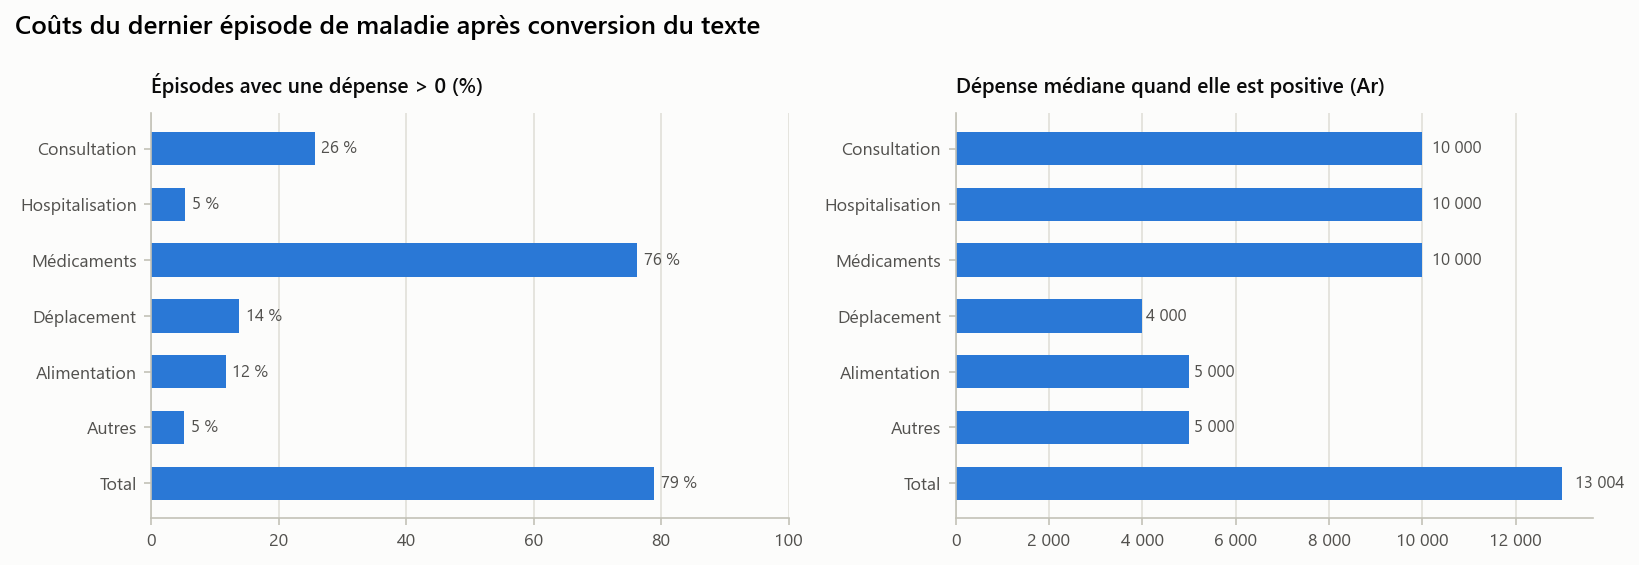
\includegraphics[keepaspectratio,alt={Coûts par poste}]{resultats/figures/couts_par_poste.png}}

\caption{Coûts par poste}

\end{figure}



Les \textbf{médicaments} forment l'essentiel de la dépense, ce qui est cohérent avec la place de l'automédication (31 \% des recours). L'hospitalisation est rare (5 \%) mais coûteuse en moyenne : elle produit la queue de distribution traitée à l'étape 1.2.



\subsection{2.5 Autres harmonisations}



\begin{itemize}

\tightlist

\item

  \textbf{Fokotany} : 237 écritures brutes \ensuremath{\rightarrow} \textbf{159 quartiers} après suppression des espaces, de la casse et des variantes d'orthographe (\texttt{Andrefatsena} \ensuremath{\rightarrow} \texttt{Andrefantsena}, \texttt{Ampivarotanomby} \ensuremath{\rightarrow} \texttt{Ampivarotan\textquotesingle{}omby}\ldots).

\item

  \textbf{\texttt{declare\_non\_malade}} : indicateur construit à partir du texte libre \texttt{type\_maladie} (\texttt{Tsy\ narary} = « je n'ai pas été malade », \texttt{0}, \texttt{Tsy\ misy}). Il concerne 262 individus et sert aux contrôles de cohérence et au traitement des manquants du bloc « dernier épisode ».

\end{itemize}



\section{3. Cohérence des données}



\subsection{3.1 Doublons}



Trois lignes sont \textbf{strictement identiques} sur les 72 variables hors identifiant (ids 3460, 3624 et 3898). Ce sont des saisies répétées du même questionnaire. On garde la première (3460) et on \textbf{supprime 3624 et 3898}. Il reste \textbf{4 074 individus}.



\subsection{3.2 Valeurs hors plage (impossibles) \texorpdfstring{\ensuremath{\rightarrow}}{->} mises à manquant, puis imputées (\texorpdfstring{\S{}}{par.} 4)}



{\def\LTcaptype{none} % do not increment counter

\begin{longtable}[]{@{}

  >{\raggedright\arraybackslash}p{(\linewidth - 6\tabcolsep) * \real{0.2500}}

  >{\raggedright\arraybackslash}p{(\linewidth - 6\tabcolsep) * \real{0.2500}}

  >{\raggedleft\arraybackslash}p{(\linewidth - 6\tabcolsep) * \real{0.2500}}

  >{\raggedright\arraybackslash}p{(\linewidth - 6\tabcolsep) * \real{0.2500}}@{}}

\toprule\noalign{}

\begin{minipage}[b]{\linewidth}\raggedright

Variable

\end{minipage} & \begin{minipage}[b]{\linewidth}\raggedright

Règle

\end{minipage} & \begin{minipage}[b]{\linewidth}\raggedleft

Valeurs

\end{minipage} & \begin{minipage}[b]{\linewidth}\raggedright

Exemples

\end{minipage} \\

\midrule\noalign{}

\endhead

\bottomrule\noalign{}

\endlastfoot

age & hors de 15--100 ans (enquête auprès d'actifs) & 4 & 3, 5, 107, 112 \\

taille\_menage & moins d'une personne & 5 & \ensuremath{-}6, 0 \\

nb\_actifs\_menage & plus d'actifs que de membres du ménage & 12 & 2 à 7 \\

budget\_alim / sante / elec & part \textgreater{} 100 \% (montant en Ariary saisi à la place d'un \%) & 12 / 11 / 9 & 5 000, 20 000, 70 000 \\

prime\_souhaitee & négative & 3 & \ensuremath{-}5 000 \\

prime\_souhaitee & entre 1 et 99 Ar (unité ambiguë : milliers d'Ariary ?) & 18 & 1, 5, 10, 40 \\

nb\_maladies\_graves & négatif & 1 & \ensuremath{-}1 \\

heures\_jour & \textgreater{} 24 h ou 0 h & 9 & 0, 406 \\

jours\_semaine & \textgreater{} 7 jours ou 0 jour & 13 & 0, 8, 13, 67 \\

anciennete\_emploi & supérieure à (âge \ensuremath{-} 5) ans & 14 & 20 ans pour un âge de 22 ans \\

jours\_arret & plus d'un an pour un épisode & 2 & 730, 3 650 \\

\end{longtable}

}



Ces valeurs sont \textbf{impossibles} ; elles sont donc mises à manquant plutôt que plafonnées. Les valeurs \textbf{possibles mais extrêmes} (365 maladies graves, ménage de 30 personnes, coût de 9,5 M Ar) sont traitées à l'étape 1.2.



\subsection{3.3 Contradictions entre questions (signalées, non corrigées)}



{\def\LTcaptype{none} % do not increment counter

\begin{longtable}[]{@{}

  >{\raggedright\arraybackslash}p{(\linewidth - 4\tabcolsep) * \real{0.3333}}

  >{\raggedleft\arraybackslash}p{(\linewidth - 4\tabcolsep) * \real{0.3333}}

  >{\raggedright\arraybackslash}p{(\linewidth - 4\tabcolsep) * \real{0.3333}}@{}}

\toprule\noalign{}

\begin{minipage}[b]{\linewidth}\raggedright

Contrôle

\end{minipage} & \begin{minipage}[b]{\linewidth}\raggedleft

Individus

\end{minipage} & \begin{minipage}[b]{\linewidth}\raggedright

Décision

\end{minipage} \\

\midrule\noalign{}

\endhead

\bottomrule\noalign{}

\endlastfoot

Déclare ne pas avoir été malade, mais au moins une maladie grave & 13 & Conservé : \texttt{nb\_maladies\_graves} est la variable cible, et la question sur le dernier épisode peut viser une autre période \\

Déclare ne pas avoir été malade, mais un coût \textgreater{} 0 & 1 & Conservé \\

Somme des trois parts de budget \textgreater{} 100 \% (chacune \ensuremath{\leq} 100 \%) & 47 & Conservé : réponses approximatives, chaque part reste plausible \\

Conjoint(e) du chef de ménage mais non marié(e) & 52 & Conservé (union libre) \\

\end{longtable}

}



Ces contradictions concernent moins de 1,5 \% des individus. Les corriger supposerait de choisir arbitrairement quelle réponse est fausse.



\subsection{3.4 Variables constantes ou faiblement informatives}



Seuil retenu : une modalité regroupe \textbf{plus de 95 \%} des individus.



{\def\LTcaptype{none} % do not increment counter

\begin{longtable}[]{@{}

  >{\raggedright\arraybackslash}p{(\linewidth - 6\tabcolsep) * \real{0.2500}}

  >{\raggedright\arraybackslash}p{(\linewidth - 6\tabcolsep) * \real{0.2500}}

  >{\raggedleft\arraybackslash}p{(\linewidth - 6\tabcolsep) * \real{0.2500}}

  >{\raggedright\arraybackslash}p{(\linewidth - 6\tabcolsep) * \real{0.2500}}@{}}

\toprule\noalign{}

\begin{minipage}[b]{\linewidth}\raggedright

Variable

\end{minipage} & \begin{minipage}[b]{\linewidth}\raggedright

Modalité dominante

\end{minipage} & \begin{minipage}[b]{\linewidth}\raggedleft

\%

\end{minipage} & \begin{minipage}[b]{\linewidth}\raggedright

Décision

\end{minipage} \\

\midrule\noalign{}

\endhead

\bottomrule\noalign{}

\endlastfoot

ancienne\_couverture & Non & 99,2 & \textbf{Exclue} \\

couverture & Non & 97,5 & \textbf{Exclue des modèles} (gardée pour la discussion de l'étape 3.3) \\

lunettes & Non & 93,9 & Conservée (sous le seuil) \\

maladie\_chronique & Non & 90,1 & Conservée : facteur de risque santé majeur malgré sa faible fréquence \\

\end{longtable}

}



Aucune variable quantitative n'est constante (écart-type \textgreater{} 0 ; la valeur la plus fréquente regroupe au plus 57 \% des individus).



\subsection{3.5 Redondances}



\begin{itemize}

\tightlist

\item

  \textbf{Variables qualitatives} : V de Cramér corrigé du biais, calculé sur toutes les paires de candidates aux modèles. \textbf{Aucune paire ne dépasse le seuil de 0,7.} Les liaisons les plus fortes restent logiques et modérées : sexe et lien avec le chef de ménage (0,61 : les chefs de ménage sont surtout des hommes, les conjointes des femmes) ; arrêt maladie et repos récent (0,59) ; statut de résidence et énergie de cuisine (0,59).

\item

  \textbf{Variables quantitatives} : la corrélation de Spearman maximale est celle entre l'âge et l'ancienneté dans l'emploi (0,70). Les deux variables sont conservées comme candidates : l'ancienneté mesure l'exposition au travail, pas seulement l'âge. Les sélections de variables des étapes 2 et 3 trancheront.

\end{itemize}



\begin{figure}

\centering

\pandocbounded{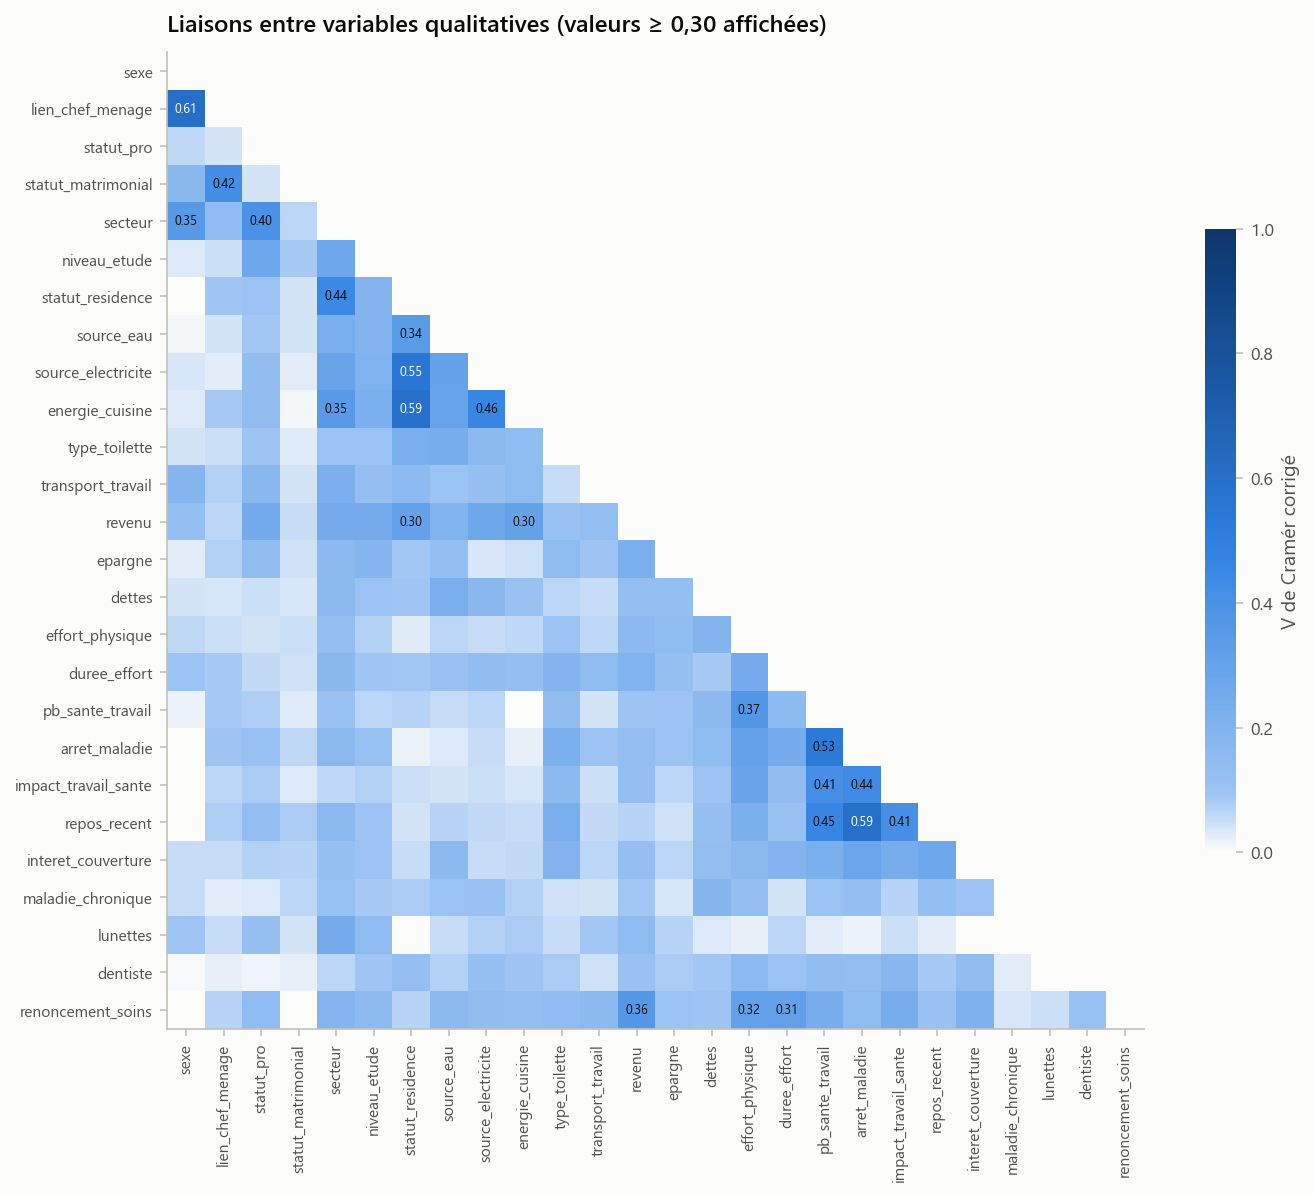
\includegraphics[keepaspectratio,alt={V de Cramér}]{resultats/figures/v_de_cramer.png}}

\caption{V de Cramér}

\end{figure}



\section{4. Valeurs manquantes : analyse et stratégie}



Le taux de manquants est mesuré \textbf{après mise au format}, c'est-à-dire en comptant aussi les textes inexploitables et les valeurs impossibles mises à manquant. Trois stratégies sont appliquées selon la nature du manque :



{\def\LTcaptype{none} % do not increment counter

\begin{longtable}[]{@{}

  >{\raggedright\arraybackslash}p{(\linewidth - 4\tabcolsep) * \real{0.3333}}

  >{\raggedright\arraybackslash}p{(\linewidth - 4\tabcolsep) * \real{0.3333}}

  >{\raggedright\arraybackslash}p{(\linewidth - 4\tabcolsep) * \real{0.3333}}@{}}

\toprule\noalign{}

\begin{minipage}[b]{\linewidth}\raggedright

Stratégie

\end{minipage} & \begin{minipage}[b]{\linewidth}\raggedright

Variables

\end{minipage} & \begin{minipage}[b]{\linewidth}\raggedright

Justification

\end{minipage} \\

\midrule\noalign{}

\endhead

\bottomrule\noalign{}

\endlastfoot

\textbf{Suppression de la variable} & 9 variables à plus de 85 \% de manquants, plus \texttt{activite\_famille} (55 \%) et \texttt{freq\_dentiste} (45 \%) & Questions \textbf{conditionnelles} (posées aux seuls malades chroniques, aux seuls assurés\ldots) : l'information utile est déjà dans la question « filtre » (\texttt{maladie\_chronique}, \texttt{couverture}, \texttt{lunettes}, \texttt{dentiste}, \texttt{secteur}). Imputer 90 \% de valeurs créerait de l'information artificielle. \\

\textbf{Imputation par la médiane} & 10 variables quantitatives (âge, ménage, budgets, ancienneté, distance, heures, jours), de 0,2 \% à 6,8 \% de manquants & Manque faible et sans structure apparente ; la médiane résiste aux valeurs extrêmes. Exemples : âge \ensuremath{\rightarrow} 37 ans (12 valeurs), heures \ensuremath{\rightarrow} 8 h (124 valeurs), distance \ensuremath{\rightarrow} 1 km (278 valeurs). \\

\textbf{Imputation par le mode} & 26 variables qualitatives, de 0,1 \% à 1,9 \% de manquants & Manque très faible (6 à 76 valeurs) : l'impact sur les distributions est négligeable. Exemples : revenu \ensuremath{\rightarrow} \texttt{100-200k} (41), renoncement \ensuremath{\rightarrow} \texttt{Oui} (76). \\

\textbf{Modalité spécifique} & \texttt{activite\_conjoint} (30 \%) & Manquant \textbf{structurel} : pas de conjoint. Modalité « Sans conjoint » si la personne n'est pas mariée, sinon « Non renseigné ». \\

\textbf{Modalité spécifique} & bloc « dernier épisode » : douleur, type de recours, satisfaction, impacts (5 à 8 \%) & Le manquant correspond souvent à l'absence de maladie : modalité « Non concerné » si l'individu déclare ne pas avoir été malade, sinon « Non renseigné ». \\

\textbf{Aucune imputation} & variables cibles : \texttt{nb\_maladies\_graves} (0,7 \%), coûts et \texttt{cout\_total} (5,0 \%) & On n'invente jamais une variable à expliquer : un individu sans valeur est simplement exclu du modèle concerné (fréquence ou sévérité). \\

\textbf{Aucune imputation} & \texttt{prime\_souhaitee}, \texttt{jours\_arret}, \texttt{distance\_soins} & Variables descriptives, non utilisées comme variables explicatives. \\

\end{longtable}

}



Le tableau complet (taux brut, taux après mise au format, traitement et nombre de valeurs imputées par variable) figure dans \texttt{tables/valeurs\_manquantes.csv}.



\section{5. Décisions par variable}



{\def\LTcaptype{none} % do not increment counter

\begin{longtable}[]{@{}

  >{\raggedright\arraybackslash}p{(\linewidth - 4\tabcolsep) * \real{0.3333}}

  >{\raggedleft\arraybackslash}p{(\linewidth - 4\tabcolsep) * \real{0.3333}}

  >{\raggedright\arraybackslash}p{(\linewidth - 4\tabcolsep) * \real{0.3333}}@{}}

\toprule\noalign{}

\begin{minipage}[b]{\linewidth}\raggedright

Décision

\end{minipage} & \begin{minipage}[b]{\linewidth}\raggedleft

Nb

\end{minipage} & \begin{minipage}[b]{\linewidth}\raggedright

Variables

\end{minipage} \\

\midrule\noalign{}

\endhead

\bottomrule\noalign{}

\endlastfoot

\textbf{Conservée --- modélisation} & 36 & sexe, age, lien\_chef\_menage, statut\_pro, statut\_matrimonial, taille\_menage, nb\_actifs\_menage, secteur, niveau\_etude, statut\_residence, source\_eau, source\_electricite, energie\_cuisine, type\_toilette, anciennete\_emploi, distance\_travail, transport\_travail, heures\_jour, jours\_semaine, revenu, budget\_alim, budget\_sante, budget\_elec, epargne, dettes, effort\_physique, duree\_effort, pb\_sante\_travail, arret\_maladie, impact\_travail\_sante, repos\_recent, interet\_couverture, maladie\_chronique, lunettes, dentiste, renoncement\_soins \\

\textbf{Conservée --- cible} & 8 & nb\_maladies\_graves ; cout\_total et ses 6 postes \\

\textbf{Conservée --- description} & 12 & fokotany, couverture, prime\_souhaitee, activite\_conjoint ; et les 8 variables du dernier épisode (douleur, jours\_arret, type\_recours, distance\_soins, satisfaction, impact\_autre, impact\_maladie\_activite, recuperation\_activite), connues seulement \textbf{après} le sinistre et donc inutilisables pour tarifer \\

\textbf{Exclue} & 18 & id ; 9 variables quasi vides (questions conditionnelles) ; activite\_famille, freq\_dentiste (redondantes et trop incomplètes) ; ancienne\_couverture (quasi constante) ; nb\_employes (17 \% de manquants, 85 \% de zéros, sans lien attendu avec le risque) ; date\_derniere\_maladie, type\_maladie, motif\_recours, benefice\_autre\_recours (texte libre ou choix multiples non exploitables) \\

\end{longtable}

}



La justification détaillée de chaque variable figure dans \texttt{tables/decisions\_variables.csv}.



\section{6. Jeu de données produit}



\textbf{\texttt{resultats/donnees\_qualite.csv}} : \textbf{4 074 individus \ensuremath{\times} 59 colonnes}. Il contient l'identifiant, les 36 variables explicatives, les 8 variables cibles, les 12 variables descriptives et 2 indicateurs (\texttt{nb\_couts\_renseignes}, \texttt{declare\_non\_malade}). Il ne reste aucune valeur manquante dans les 36 variables explicatives ; les variables cibles gardent leurs manquants (28 pour la fréquence, 205 pour le coût total), de même que les variables descriptives (\texttt{prime\_souhaitee} 157, \texttt{jours\_arret} 181, \texttt{distance\_soins} 204).



{\def\LTcaptype{none} % do not increment counter

\begin{longtable}[]{@{}lrrrrr@{}}

\toprule\noalign{}

Variable convertie & n & Médiane & Q3 & P99 & Max \\

\midrule\noalign{}

\endhead

\bottomrule\noalign{}

\endlastfoot

anciennete\_emploi (ans) & 4 074 & 10 & 19 & 37 & 50 \\

distance\_travail (km) & 4 074 & 1,0 & 2,0 & 10 & \textbf{510} \\

heures\_jour & 4 074 & 8 & 8 & 24 & 24 \\

jours\_semaine & 4 074 & 6 & 6 & 7 & 7 \\

jours\_arret & 3 893 & 3 & 5 & 60 & 365 \\

distance\_soins (km) & 3 870 & 0,5 & 2,0 & 9 & 92 \\

cout\_total (Ar) & 3 869 & 8 000 & 23 000 & 500 000 & \textbf{9 500 000} \\

\end{longtable}

}



Les maxima (en gras) confirment le besoin d'un traitement des valeurs aberrantes.



\ensuremath{\rightarrow} Suite : \href{../1.2_aberrantes/README.pdf}{étape 1.2 --- Valeurs aberrantes}



\section{Fichiers produits}



{\def\LTcaptype{none} % do not increment counter

\begin{longtable}[]{@{}

  >{\raggedright\arraybackslash}p{(\linewidth - 2\tabcolsep) * \real{0.5000}}

  >{\raggedright\arraybackslash}p{(\linewidth - 2\tabcolsep) * \real{0.5000}}@{}}

\toprule\noalign{}

\begin{minipage}[b]{\linewidth}\raggedright

Fichier

\end{minipage} & \begin{minipage}[b]{\linewidth}\raggedright

Contenu

\end{minipage} \\

\midrule\noalign{}

\endhead

\bottomrule\noalign{}

\endlastfoot

\texttt{resultats/donnees\_qualite.csv} / \texttt{.xlsx} & \textbf{Jeu nettoyé} (entrée de l'étape 1.2) \\

\texttt{tables/decisions\_variables.csv} & Décision et justification pour chacune des 74 variables \\

\texttt{tables/valeurs\_manquantes.csv} & Manquants avant / après, stratégie, valeurs imputées \\

\texttt{tables/reponses\_multiples.csv} & Cellules à réponses multiples par variable \\

\texttt{tables/recodage\_modalites.csv} & Correspondance réponse brute \ensuremath{\rightarrow} modalité finale \\

\texttt{tables/conversion\_texte\_nombre.csv} & Bilan de la conversion texte \ensuremath{\rightarrow} nombre \\

\texttt{tables/couts\_par\_poste.csv} & Synthèse des six postes de coût \\

\texttt{tables/controles\_plages.csv}, \texttt{contradictions.csv} & Contrôles de cohérence \\

\texttt{tables/dominance\_modalites.csv} & Part de la modalité dominante (variables quasi constantes) \\

\texttt{tables/v\_de\_cramer.csv}, \texttt{paires\_v\_de\_cramer.csv}, \texttt{paires\_spearman.csv} & Redondances \\

\texttt{tables/stats\_variables\_converties.csv} & Statistiques des variables converties \\

\texttt{resultats/figures/*.png} & V de Cramér, coûts par poste \\

\texttt{resultats/journal.txt} & Sortie complète du script \\

\end{longtable}

}



\end{document}

